%!TEX root = ../Thesis.tex
\chapter{More about HPC systems at CSC}
This Chapter gives more information about the HPC systems at CSC, on top of Section \ref{sec:hpc}, including the overview of CPU for Mahti, more details about the AMD MI250X GPU, and how the hardware is connected for each HPC system.

\section{Mahti CPU}
The NUMA configuration of Mahti \cite{mahti} involves a hierarchical structure within each node. Each node contains two sockets, each accommodating a single CPU alongside memory DIMMs. Although the memory within the node is shared, the performance of memory access varies based on the proximity of the core to the memory. Mahti operates each CPU in NPS4 (NUMA per socket 4) mode to optimize memory performance, dividing each CPU into four NUMA domains. Each NUMA domain includes 16 cores and two memory controllers, providing 32 GiB of memory. Thread allocation within each core follows a specific pattern: core 0 runs threads 0 and 128, core 1 runs threads 1 and 129, and so forth. Figure \ref{fig_mahti_numa} shows how the threads are distributed over each core and NUMA node.

\begin{figure}[H]
    \centering
    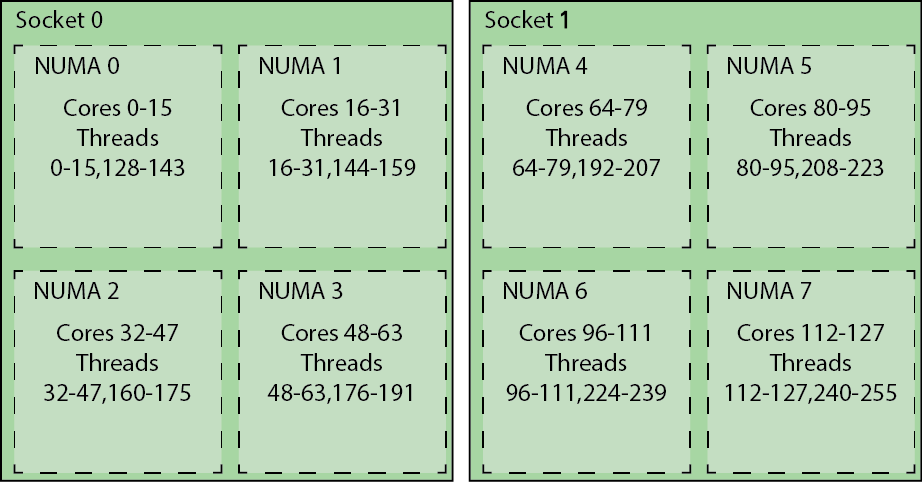
\includegraphics[width=0.8\textwidth]{figures/mahti_numa.png}
    \caption{Mahti NUMA structure overview \cite{mahti}}
    \label{fig_mahti_numa}
\end{figure}

Each core possesses 32 KiB of L1 data cache, 32 KiB of L1 instruction cache, and a private 512 KiB L2 cache. Additionally, each core has two FMA (fused multiply-add) units capable of processing operations on full 256-bit vectors. Consequently, each unit can execute operations on 8 single-precision floats or 4 double-precision floats per clock cycle, resulting in 16 double-precision floating point operations per clock cycle.

As shown in Figure \ref{fig_mahti_ccd}, cores in the CPU are grouped into core complexes (CCXs) and further combined into compute dies (CCDs). At the CCX level, four cores share a 16 MiB L3 cache within the CCX, and two CCX parts combine to form a compute die (CCD).

\begin{figure}[H]
    \centering
    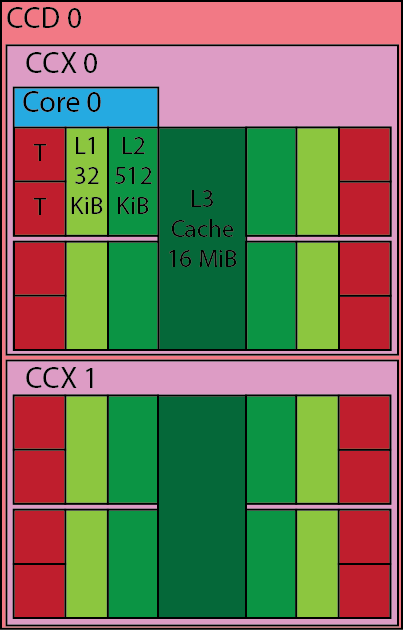
\includegraphics[width=0.3\textwidth]{figures/mahti_ccd.png}
    \caption{Mahti CCD structure overview \cite{mahti}}
    \label{fig_mahti_ccd}
\end{figure}

Each processor comprises eight compute dies and an additional I/O die, including memory and PCI-e controllers. Furthermore, each node consists of two processors and one 200 Gbps HDR network adapter, as shown in Figure \ref{fig_mahti_node}.

\begin{figure}[H]
    \centering
    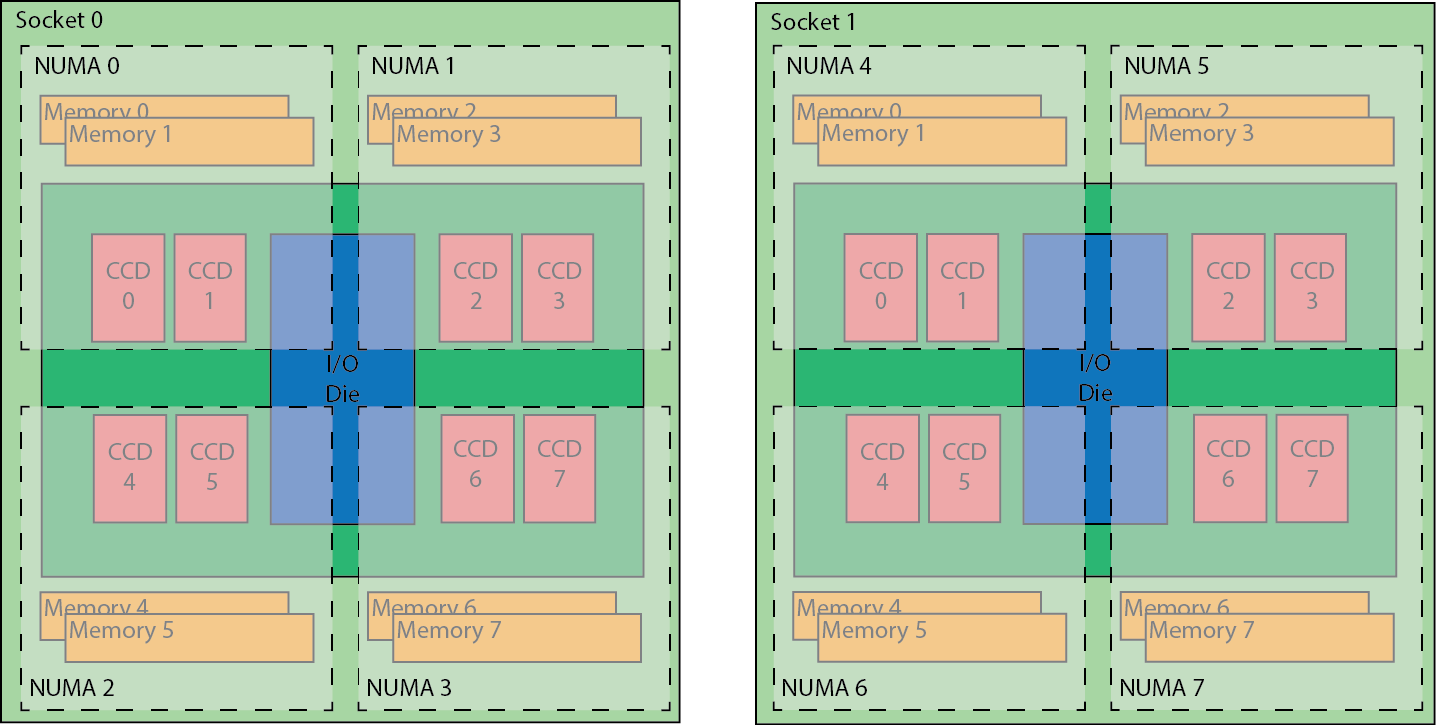
\includegraphics[width=1.1\textwidth]{figures/mahti_node.png}
    \caption{Mahti node structure overview \cite{mahti}}
    \label{fig_mahti_node}
\end{figure}

\section{AMD MI250X GPU}

\begin{figure}[H]
    \centering
    \includesvgpath[width=1.1\textwidth]{mi250x-gcd.svg}
    \caption{AMD MI250X GCD structure \cite{lumi}}
    \label{mi250x-gcd.svg}
\end{figure}

The GCD structure of AMD MI250X GPU is demonstrated in Figure \ref{mi250x-gcd.svg}. When a kernel is dispatched for execution on the GPU, it is organized as a grid of thread blocks (workgroups), with the grid and thread blocks being one, two, or three-dimensional. The grid can have a maximum number of blocks specified along each dimension of (2147483647, 2147483647, 2147483647), while the maximum number of threads (work-items) for each dimension of a block is (1024, 1024, 1024), with a thread block size limit of 1024, which means size.x * size.y * size.z must be less or equal to 1024.

The thread blocks are assigned to one of the 110 compute units and are scheduled in groups of 64 threads, known as wavefronts. This is analogous to a warp on NVIDIA hardware, except that a warp consists of 32 threads, while for AMD hardware, a wavefront comprises 64 threads.

The execution process of wavefronts by a compute unit can be outlined as follows:

\begin{enumerate}
    \item Each wavefront has 64 work items (threads) allocated to one of the  16-wide SIMD units.
    \item Most instructions are executed within a single cycle, although one instruction requires four cycles per wavefront.
    \item With 4 SIMD units available per compute unit, up to 4 wavefronts can be processed simultaneously, ensuring a consistent throughput of one instruction per wavefront per compute unit.
\end{enumerate}

Figure \ref{mi250x-compute-unit.svg} shows that each compute unit has 512 64-wide 4-byte vector general-purpose registers. Additionally, the unit provides access to low-latency storage through a 64 kB local data share (LDS, shared memory), accessible to all threads within a block. The programmer manages the LDS allocation. Furthermore, each compute unit has access to 16 kB of L1 cache.

\begin{figure}[H]
    \centering
    \includesvgpath[width=1.1\textwidth]{mi250x-compute-unit.svg}
    \caption{AMD MI250X compute unit structure \cite{lumi}}
    \label{mi250x-compute-unit.svg}
\end{figure}

The vector ALUs are complemented by matrix cores optimized to execute matrix-fused multiply-add instructions. These cores offer significant acceleration for generalized matrix multiplication computations, which is crucial for linear algebra in High-Performance Computing applications and AI workloads. Each compute unit (CU) has four matrix cores capable of achieving a throughput of 256 double-precision floating-point format (FP64) Flops/cycle/CU.

\section{Connections}
This Section introduces how the hardware or node is inter-connected, for the three HPC systems at the CSC: Puhti, Mahti, and LUMI.

\subsection{Puhti}
The Puhti\cite{puhti} interconnect architecture is based on a dual-rail Mellanox HDR100 InfiniBand setup. It offers a non-blocking fat-tree topology with a blocking factor of approximately 2:1 and delivers an impressive aggregate bandwidth of 200 Gbps, ensuring efficient connectivity across the network.

\subsection{Mahti}
The network interconnect in Mahti is based on Mellanox HDR InfiniBand, with each node connected via a single 200 Gbps HDR link. The network topology adopts a dragonfly+ configuration, in which multiple groups of nodes are internally connected using a fat tree topology. These fat trees are interconnected using all-to-all links to ensure fully non-blocking connectivity between groups, as shown in Figure \ref{fig_mahti_df_ex}.

\begin{figure}[H]
    \centering
    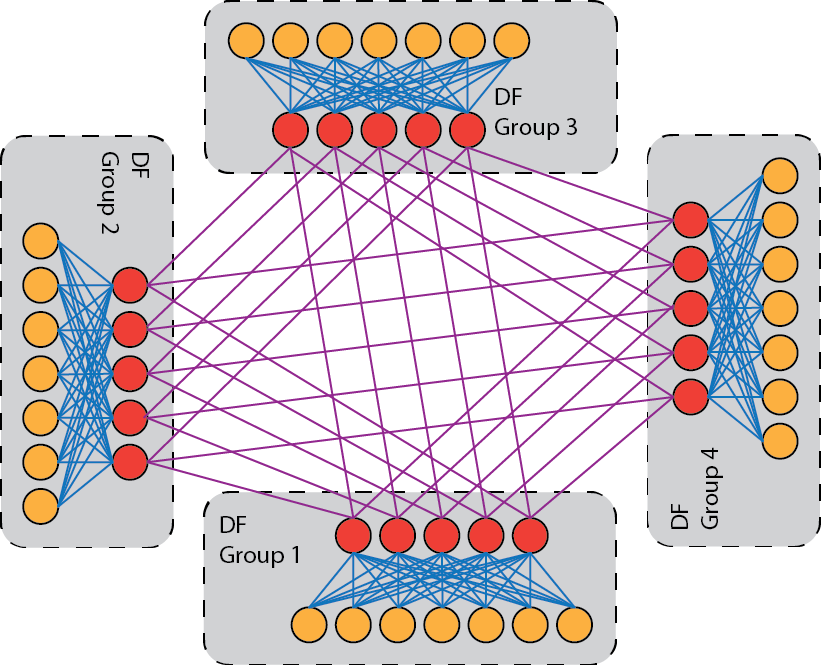
\includegraphics[width=0.8\textwidth]{figures/mahti_df_ex.png}
    \caption{Mahti dragonfly+ configuration overview \cite{mahti}}
    \label{fig_mahti_df_ex}
\end{figure}

In Mahti, each dragonfly group comprises 234 nodes, with an internal fat tree featuring a blocking factor of 1.7:1 and 20 or 18 nodes connected per leaf switch. Each leaf switch connects to the spine switch in the group via 12 200 Gbps links. Figure \ref{fig_mahti_df} shows the topology of such a group. There are six groups, with five 200 Gbps links connecting each spine switch to a spine switch in every other group, facilitating comprehensive inter-group communication.

\begin{figure}[H]
    \centering
    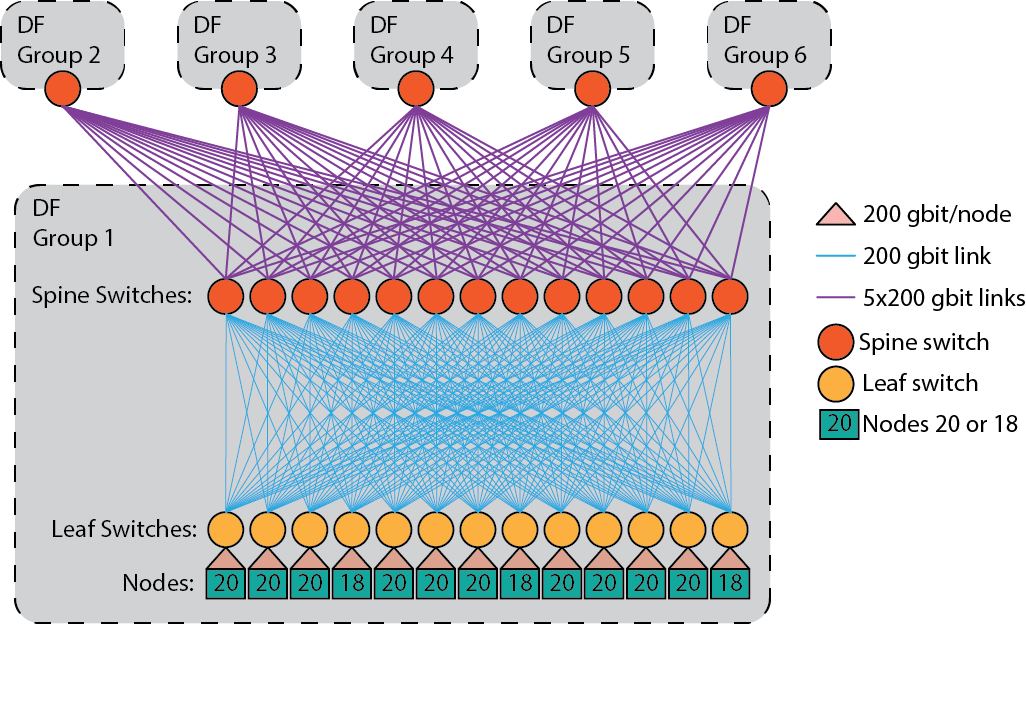
\includegraphics[width=1\textwidth]{figures/mahti_df.png}
    \caption{Mahti dragonfly topology \cite{mahti}}
    \label{fig_mahti_df}
\end{figure}

\subsection{LUMI}
Figure \ref{fig_lumig_topology} shows the node LUMI topology. Each MI250X module includes 5 GPU-GPU links, 2 CPU-GPU links, and 1 PCIe link to the slingshot-11 interconnect. The MI250X modules are connected via an in-package Infinity Fabric interface, capable of delivering a theoretical peak bidirectional bandwidth of up to 400 GB/s. Furthermore, GCDs across different MI250X modules are linked through single or double Infinity Fabric links, offering peak bidirectional bandwidths of 100 GB/s and 200 GB/s, respectively. Each MI250X module directly connects to the slingshot-11 network, affording peak bandwidths of up to 25+25 GB/s. 

\begin{figure}[H]
    \centering
    \includesvgpath[width=1.1\textwidth]{lumig-node-overview.svg}
    \caption{LUMI GPU node topology overview \cite{lumi}}
    \label{fig_lumig_topology}
\end{figure}

Figure \ref{fig_lumig_cpu_gpu_links} shows the CPU-GPU links from a CPU-centric or GPU-centric point of view of the LUMI GPU node. Proper binding of the NUMA node to the GPU can be essential to ensure optimal application performance.

\begin{figure}[H]
    \centering
    \includesvgpath[width=1.1\textwidth]{lumig-cpu-gpu-links.svg}
    \caption{CPU-GPU links on LUMI GPU node \cite{lumi}}
    \label{fig_lumig_cpu_gpu_links}
\end{figure}
